\documentclass[free]{flammie}

\usepackage{graphicx}

\title{Keeping Up Appearances---or how to get all Uralic languages included into
bleeding edge research and software: generate, convert, and LLM your way into
multilingual
datasets\footnotepubrights{\aclanthologypostprintdoi{2024.iwclul-1.16}}}
\author{Flammie A Pirinen\\
Divvun\\
UiT---Norgga árktalaš universitehta\\
Tromsø, Norway\\
\url{flammie.pirinen@uit.no}}
\date{\today}

\begin{document}

\maketitle

\begin{abstract}
    The current trends in natural language processing strongly favor large
    language models and generative AIs as the basis for everything.  For Uralic
    languages that are not largely present in publically available data on the
    Internet, this can be problematic.  In the current computational linguistic
    scene, it is very important to have representation of your language in
    popular datasets.  Languages that are included in well-known datasets are
    also included in shared tasks, products by large technology corporations,
    and so forth.  This inclusion will become especially important for
    under-resourced, under-studied minority, and Indigenous languages, which
    will otherwise be easily forgotten.  In this article, we present the
    resources that are often deemed necessary for digital presence of a language
    in the large language model -obsessed world of today.  We show that there
    are methods and tricks available to alleviate the problems with a lack of
    data and a lack of creators and annotators of the data, some more successful
    than others.
\end{abstract}

\section{Introduction}

In recent years, the landscape of language technology has changed quite rapidly,
mainly with the advent large language models, but the overarching shift towards
big data has been ongoing for longer.  The problem with this shift is, that it
is based on the big data for large majority languages, the inclusion of all the
smaller languages, including all of the Uralic languages, has come as an
afterthought if at all.

The expected solution for the continued sustainability of minority Uralic
languages in the landscape of modern languages in the time of large language
models is to ``generate'' more data.  Ideally, by `generate', the engineers in
large language model contexts mean, that authentic written (or spoken) data
needs to be created by native writers who should not make too many spelling or
grammar errors and write the most current normative form.  This can be an
unreachable goal for a language that has fewer than million speakers and writers
who are not L1, as while the requirements for large language models are going
down over time, they are still orders of magnitude larger that can plausibly be
created by limited amount of writers and speakers in limited amount of time.

What we suggest in this paper is to carefully organise the initial work of
corpus curation and creation around materials that are of high importance to the
contemporary language technology community.  We leverage existing resources and
language technologies to minimise unnecessary and repetitive work by linguists
and language professionals on the language data that is being worked on;
automating what can be automated and re-using linguists annotation efforts is a
key to efficient development of high-quality human verified gold data.

Our \textit{research question} is, going from existing langauge technology
resources: which tools are best suitable for launching and bootstrapping which
resources. If language has usable electronical dictionaries, morphological
analysers and generators, spell-checkers and so on, what can be used to
effectivise the dataset creation and corpus curation. The question is especially
interesting now, as there is a possibility to use contemporary multilingual
large language models, as well as traditional rule-based, statistical and hybrid
language models to perform various pre-processing and processing tasks.

Our \textit{key contributions} from this article are: \textit{the experimental
framework} for others to compare and combine methods of gold data annotation for
smaller languages, the \textit{pipelines} from traditional rule-based
annotations and LLM generations into concrete target formats, and the results of
comparing some of the approaches for a low resource Uralic language along with
recommendations of what is currently the most effective approach. As a side
product we have created, curated and annotated beginnings of \textit{several new
datasets} for an under-resourced Uralic language.

We have laid out experimental computational linguistics data creation and
annotation system that can use both existing rule-based tools as well as large
language models to aid the processs.  One of the goals of this experiment and
the approach is that we want to promote inclusion of more Uralic languages in
all of the common language technology datasets.  We are considering three
separate approaches to help creation of annotated gold data:

\begin{enumerate}
    \item rule-based generators and generative language models to generate a
        starting point for a data set, to be proof-read and re-annotated by
        humans,
    \item rule-based analysers creating annotated dataset in legacy and ad hoc
        formats that are converted and organised into a starting point for human
        re-annotation, and
    \item generative language models providing human annotators with starting
        points or improvements during annotation process
\end{enumerate}

There are of course other possibilities as well, these are based on our previous
experience and iterations with different datasets and projects. It must be noted
that the goal here is to generate something comparable to human annotated gold
corpus, so we are not planning to automate data generation or annotation. This
has to be also contrasted to the reality of limited human resources for working
with smaller Uralic languages, we do not necessarily have a possiblity to hire 5
annotators to work on data full hours for several months, but to ask if the
language experts who have other main jobs as language experts can use hours or
two here and there on the task, this is one of the motivations of our experiment
as well.

\section{Background}

The Uralic languages, especially besides the bigger national languages, are
relatively under-resourced; the size of freely available texts is measured in
millions of tokens or less.  However, Uralic languages do have strong traditions
of rule-based language technology.  Also, lately, the large language model
-based language technology has showed itself as a viable option for some use
cases.  Our approach to resource creation to overcome some of the
under-resourcedness problem is thus to see if we can leverage the existing
technology to supplement the well-planned tactical selection of language dataset
resources.  In this article, we suggest curating and creating data that are
highly relevant for the large language model building industry and also for the
researchers of languages in language technology and linguists as well.  While
majority of industry and researchers concern themselves with basically English
and maybe handful of commercially plausible majority languages of the world, we
have discovered some related research both from the industry and the researchers
who specialise in minority and under-resourced languages.

As one reference point, we study what technology companies and central research
groups in LLM-based language technology have said about support for smaller
language in the recent years; One reason for writing this article and its
experiments is also inspired by these works: Meta and FAIR research group
(Facebook's AI Research) have released resources and studies under the moniker
of \textit{No language left behind}~(NLLB)~\cite{nllb}, also known for datasets
and evaluation schemes under \textit{Scaling neural machine translation to next
200 languages}~(FLoRES)~\cite{flores}. Unsurprisingly, this data set has so far
included only Finnish, Estonian, and Hungarian when it comes to Uralic language
inclusion.  Alphabet and Google research have also been active on extending the
range of languages supported under the name of \textit{next 1000
languages}~\cite{bapna2022buildingmachinetranslationsystems}. They have also
published several research papers listing exactly the sources they use to gather
information and data on the languages \cite{ritchie-etal-2024-linguameta}, this
is directly useful information to know that, if you want to be included in
Google's considerations list of languages that might be supported or relevant,
perhaps you want to have data in the resources and datasets they use.

The resources that we use in this articles experiments here have also been used
for several years now in the academic community as the go-to resource to measure
if your tool works with the given language.  For example, the \textit{Universal
Dependencies} (UD) treebanks~\cite{ud214}, are used in a huge number of papers
investigating computational linguistic methods in a large number of languages,
including the annual shared tasks in syntactic parsing.  It would thus appear
that UD as a resource has passed the test of time.  Secondly we have seen the
\textit{Unimorph} dataset, that concerns morphology of languages, has been used
widely in the research and applications. Namely with research of morphophonology
and machine learning there have been regular shared tasks.
%Finally, the resource that is often asked for and we think is well suited for
%these experiments is named entity corpus.
We have explicitly left out parallel corpora and machine translations from this
article for two reasons: firstly it is already a main focus of the large
corporations and research groups working on the natural language engineering
tasks and secondly our corpus selection is based on aiming to have a large
subset of professionally human-translated texts as the source texts in these
datasets, we find these are much more valuable than machine translated or
post-edited texts, for the early phases of big data building we are in.

For the experimentation of this article I have chosen Inari Sámi as a target
language; Inari Sámi is a Uralic language, that does not as of now have many of
the resources that we are about to create.  It is a low-resource Indigenous
language with limited amount of speakers and written resources available, but an
active speaker community that writes new texts.  We have existing tools in
rule-based language technology available from the well-known free and open
source repository\footnote{\url{https://giellalt.github.io/lang-smn}}.
Furthermore, the most recent versions of large language model -based systems
have been seen to support Inari Sámi (instead of just refusing to handle it and
deferring to professionals as earlier versions did).  Finally, we have a
computational linguist who is not a native speaker but is capable of working
with the language and has contacts to language experts, we find this is
sufficient for initial experimentation, but of course for serious language data
building, more expert knowledge is needed.

For some the work on dataset creation there has been previous works, for example
in Universal Dependencies and rule-based analyser there are existing methods
that have been used for other existing uralic dependencies treebanks, such as
the North Sámi~\cite{tyers-sheyanova-2017-annotation} and Karelian
treebanks~\cite{pirinen2019building}. For generation of the UniMorph data, some
of the datasets are generated based on rule-based generators~\cite{unimorph},
strictly speaking Wiktionary can also be considered as rule-based morphological
generation, however, we have not found this mentioned explicitly in existimg
articles about unimorph.


\section{Methods}

Our experimentation concerns the use of existing language technology tools to
help the creation of the datasets while following the rules and ideals behind
the given datasets.  For example, when Universal Dependencies guidelines
dictates that the dependency annotation must be manual or human made, we do not
use the tools to generate unchecked 1-best annotations that would pollute the
dataset.  The most common strategy here is to give all plausible hypotheses from
the automatic analysis to the linguist to post-edit, but another option is that
the post-edited analyses are verified to be plausible analyses of the system
(our end goal is to have a gold standard that agrees with the analyser and
linguistic expertise).

For the existing rule-based systems, we have downloaded and installed well-known
GiellaLT softwares, which are freely available from the GitHub with an open
source
licence~\cite{pirinen2023giellalt}.\footnote{\url{https://giellalt.github.io}}
The LLM experimentation is performed using a ChatGPT, the state-of-the-art
chatbot interface to a closed-source, commercial neural network.\footnote{The
version tested at the time of writing identifies itself as GPT-4, which was the
newest model at the time we began experimenting but has probably been outdated
by the time of the publication.} We have chosen ChatGPT since it is the most
popular one, it has freely usable version available for most Uralic language
researchers even without expensive AI budget.  An example of ChatGPT performing
UniMorph dataset generation task can be seen in Figure~\ref{fig:chatuit}.

\begin{figure}
    \centering
    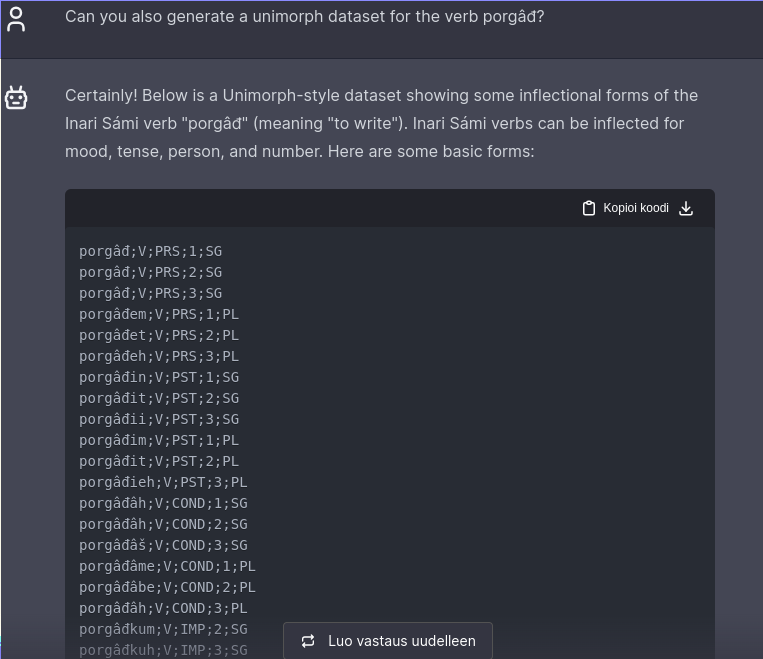
\includegraphics[width=\columnwidth]{chatuit.png}
    \caption{ChatGPT generating data for Inari Sámi UniMorph dataset.\label{fig:chatuit}}
\end{figure}

When working with a preexisting computational linguistic, rule-based system, one
of the main engineering efforts lies on the conversion. Although it sounds
trivial, there is a lot of linguistic and engineering work to be taken into
account here: the actual format of the analyses is rarely exactly the same, so a
mapping needs to be devised, for example, converting ``noun'' analyses from
\texttt{+N} to \texttt{N;} or \texttt{NOUN}. The mappings can also be 1:n or
m:1, merging and joining `tags', as well as more involved re-writings.  There
are a lot of other technical minor details related to such generations and
conversions that are beyond the scope of this article, for example, we needed an
algorithm that could remove duplicate forms that is aware of Unicode
normalisation forms and folding to avoid having the linguist read word forms
that look exactly the same several times.  The topic of conversions in itself is
large enough to deserve its own article,\footnote{we have attempted to write one
such article, even at very condensed format it easily exceeds 8 pages that is
the maximum for average conference article in language technologies.} for the
purposes of this article we will point the readers to our github repositorium
containing freely available scripts.\footnote{\url{anonymised}} Some examples of
conversions are given in the Figure~\ref{fig:conversions}.

\begin{figure*}
E.g. \textit{Finite State Morphology} to \textit{Unimorph}
    \begin{verbatim}
táálu      táálu+N+Sg+Nom               <-> táálu      táálu   N;SG;NOM
táálust    táálu+N+Sg+Loc               <-> táálust    táálu   N;SG;LOC
tálustân   táálu+N+Sg+Loc+PxSg1         <-> tálustân   táálu   N;SG;LOC;PSS1S
    \end{verbatim}
E.g. \textit{VISL CG 3} to \textit{Universal Dependencies}
\begin{verbatim}
"<mun>"
    "mun" Pron Pers Sg1 Nom @SUBJ> #1->2
:
"<juuhim>"
     "juuhâđ" <mv> V TV Ind Prt Sg1 @FMV #2->0
:
"<vuolâ>"
    "vuolâ" N Sem/Drink Sg Acc @<OBJ #3->2
                                      ^^^
                                      |||
                                      vvv
# textid = example.1
# text = mun juuhim vuolâ
1	mun	mun	PRON	Pron Pers	Case=Nom|Number=Sing|Person=1|PronType=Pers	2	nsubj	_ _
2	juuhim	juuhâđ	VERB	V TV	Mood=Ind|Number=Sing|Person=1|Tense=Past	0	root	_ _
3	vuolâ	vuolâ	NOUN	N Sem/Drink	Case=Acc|Number=Sing	2	obj	_ _
\end{verbatim}
    \caption{Conversions between traditional rule-based analyses and target dataset formats
    \label{fig:conversions}}
\end{figure*}

The experiments with LLMs are based on the currently available free ChatGPT
interface prompted in English. We begin prompting with the most straightforward
requests, e.g. ``can you generate a unimorph annotated list of all word-forms
Inari Sámi noun táálu?'', ``create a CONLL-U annotated version of this
sentence'', etc.

It might be noteworthy, that since our goal is inclusion of our Uralic languages
in the relevant datasets, there is also a component of social engineering
involved in all of the dataset creations.  Merely producing text files that
contain acceptable data is only a first step.  The datasets we have selected to
experiment with, the selection has been also based on the openness and
documentation of the contribution process; all of the given datasets exist on
GitHub, and the contribution process is detailed in the documentation and
happens largely over GitHub only. This is in contrast to the commercially backed
datasets mentioned earlier; while it would be very valuable to have all Uralic
languages in the \textit{No Languages Left Behind} and \textit{Next Thousand
Languages}, the way to contribute here is not immediately so obvious and
available to larger audiences.

\section{Corpora and Data Selection}

The corpora available for low-resource Uralic languages are scarce and limited.
The whole corpora of publically available web crawl data is typically less than
the millions of tokens that is often advertised as minimum requirement of large
language models.  Furthermore, the data that is available is limited by
licences, quality, and genres: While some argue that all data that can be
crawled is free to use for language technologies, in practice ethical use
requires selecting only the data that has explicitly been licenced with a
suitable licence, such as Wikipedia or data coming from governmental public
domain records---or that has been personally licenced with the author for the
specific use.  That furthermore limits both quality---wikipedia data is written
by language learners---and genres---government's publication are mainly
politics, healthcare and such.

In this experiment we have used primarily freely licenced data from Saami
international corpora (SIKOR),~\cite{sikor_06.11.2018} but we have also
performed a short experiment on self-created and self-translated data that large
language model should not contain from beforehands.

\section{Experimental results}

The main results of our experiment will be the actual datasets we can produce.
To quantify the usefulness of the langauge technology tools we have measured
post-edit distances.  We have also performed a linguistic error analysis to
quantify the errors made, the effect on the time/effort tradeoff is further
discussed in the Section~\ref{sec:discussion}.

In our experiment in creating datasets for Unimorph, we used both the rule-based
system and the LLM to generate the full datasets, that can be read and corrected
by a human.  The results of generating are shown in the
table~\ref{table:unimorphs}.  The expected forms is based on the linguistic
grammars we have available~\cite{morottaja2023inarinsaamen}.  We have measured
the numbers of forms generated, Coverage counted as proportion of generated
unique forms out of expected and Accuracy as proportion of fully correct forms
and analyses of all generated.  In general rule-based approach is close to the
gold standard, which is expected from rule-based systems, the LLM has also
generated a smaller subset of forms with lower accuracy.

\begin{table*}[]
    \centering
    \begin{tabular}{lrrrrrrrr}
    \toprule
        POS & \bf Expected & \bf RB & \bf RB & \bf RB & \bf LLM & \bf LLM &  \bf LLM \\
            & \bf forms & \bf forms & \bf Cov~\% & \bf Acc~\% & \bf forms & \bf Cov~\% & \bf Acc~\% \\
    \midrule
     \bf Nouns   & 58 & 100$^*$ & 100~\% &       & 14 & 15~\% & 21~\%\\
     \bf Verbs   & 57 & 55      & 96~\%  & 99~\% & 22 & 39~\% & 0~\% \\
     \bf Adjectives & 51 & 61 & 100~\%   &       & 14 & 20~\% & 10~\% \\
    \bottomrule
    \end{tabular}
    \caption{Unimorph dataset creation statistics. Expected forms is number of
    forms based  on the grammar, RB from rule-basd generator and LLM from large
    language model, Coverage and Accuracy measured in \% units. $^*$ Some extra
    forms in rule-based model are due to allomorphy which was not accounted for
    expected forms.\label{table:unimorphs}}
\end{table*}

In our experiments in Universal Dependencies annotation, we used the rule-based
system to generate ambiguous listing of all potential readings of the sentence
with annotations, according to the guidelines in previous works
by~\cite{pirinen2019building}, and asked LLM to generate similar hypotheses
likewise.  In Table~\ref{table:ud} we measure the post edit distance of the
sentences fixed and re-annotated, the error rates are calculated as
$E=\frac{S+I}{N}$, where $E$ is the error rate, $S$ is number of substitutions
made, $I$ is the insertions made, and $N$ number of readings (i.e. N is number
of CONLL-U lines with an index). We do not have $D$ for deletions since both
methods generated correctly generated one token per token in the input and there
are so far no retokenisation requirements (multi-word tokens, multi-token words
etc.), however LLM missed some punctuation tokens causing an insertion to be
required. The full error rate basically counts whole lines of CONLL-U when
making matches and dep error rate just the dep field.

\begin{table}[]
    \centering
    \begin{tabular}{lrr}
    \toprule
    System & \bf Full WER & \bf Dep WER \\
    \midrule
    \bf Rule-Based & 0.47 & 0.22 \\
    \bf LLM  & 1.00 & 0.52 \\
    \bottomrule
    \end{tabular}
    \caption{Caption\label{table:ud}}
\end{table}

\section{Discussion}\label{sec:discussion}

We have tested rule-based and LLM-based annotations as a help in linguistic
work.  Currently, for morphology we get clearly better results with the
rule-based tools and the results are good enough that it makes work on dataset
creation more effective.  If we analyse the errors that the systems make, we see
that rule-based system includes some results with linguistically motivated
potential errors, like wrong stem alternation or missing accent in a suffix.
The errors in LLM generated version are that it just uses seemingly random
suffixes with unchanged stem, it also uses some forms like cases that do not
exist in Inari Sámi (but for example exist in Finnish), all in all cleaning this
data would possible even be slower than writing the data by hand.  When we
error-analyse the dependency analysis the results get more interesting, like
both starting points require quite a significant amount of work to get to
gold-standard state, but this is also to be expected if reference the past
experiences of UD annotation from converted or machine analysed starting point.
What is interesting is that the LLM can sometimes generate quite accurate
depdendency subgraphs of certain expressions, for example personal names, we
assume this is due to them appearing in very similar form in existing English
documentations, where high level dependency structure is the same even if there
are slight variations in the morphological level.

There are a large number of different large language models and generative
artificial intelligence that could possibly be used to experiment this and that
is a common feedback we get.  We are using a version of a popular LLM that is
available to us, without excessive extra costs.  This is also available to most
researchers who are the target audience of this paper.

A common feedback we get, that there are various techniques that should be used
for low resource setup, like fine-tunings, transfer learnings,  in context
learnings, prompting techniques and so on.  We are experimenting in a situation
where we start with zero data for the fine-tuning task, we are the ones who will
create these data initially, so the use of such data will generally be a future
research topic, after we have done the initial data creation.  As the
methodology here is extremely fast moving and outdates itself in matter of
months, we try to begin by only importing either approaches that have been
proven and stabilised, perhaps in majority language context, into out lesser
resourced languages, or we can perform experimentation that does not tie up too
much valuable and scarce resources.  Another interesting future research
question would be whether it is more beneficial and time-effective to fine-tune
early or on-goingly, given the constraints in data and human resources we face
in the processing of smaller Uralic languages.  We have not found an easy enough
recipe to do transfer learning that would not take us more time than actually
working on the data creation as described by the approach of this article.  Our
impression is furthermore that there is currently ongoing research on this topic
that we hope will yield some answers that are relevant to us as well.


It is exciting to see that, even if the large language models have rathar
disappointing accuracy in generating and annotation of smaller Uralic languages,
they are able to generate something that is relevant to the task and
occasionally some word-forms or annotations are even correct.  This suggests
that maybe with further fine-tuning, prompting, in-context learning, transfer
learning, and so forth, there could be a usable version of LLM-aided language
data annotation and generation in the future.

One question for future work is of course how to integrate these findings to a
workflow and softwares for annotation.  In this experiment we used normal text
editors and raw data formats for data annotation, which is suitable for
programmers and short experiments, for the full scale linguistic annotation this
would be integrated to a specific editor.  And that raises the question of if
the ideal way to help linguistic jobs would bear a user interface similar to
what we get in the email post writing programs, office tools and programming
editors today with a so-called \textit{co-pilot}?


\section{Conclusion}

We performed several experiments to find out an efficient way of creating NLP
datasets for smaller Uralic languages.  We have found that using both existing
rule-based technology and large language models can help rapid creation of the
data, but neither approach is without its caveats.  The gold standard remains
fully human annotated data, but in lack of that it should be considered if we
can achieve reasonable amounts of resources with computer-aided annotation
modes.

\section*{Limitations}

The experimentation on large language models is done using one closed source
commercial system and is not reproducible at all, however, this is a common
practice in the science of natural language processing in 2024.

The experiments were performed by language learner instead of native speaker or
expert, the qualitative results may differ when language experts are working on
the same pre-processed data.

\section*{Ethics}

The large language models used in this experimentation have wasted an estimated
several hundreds of litres of drinking
water~\footnote{\url{https://www.thetimes.com/uk/technology-uk/article/thirsty-chatgpt-uses-four-times-more-water-than-previously-thought-bc0pqswdr}}
and not insignificant amount of
energy~\cite{strubell2019energy}.\footnote{\url{https://disconnect.blog/silicon-valley-is-sacrificing-the-climate-for-ai/}}
If LLM method is taken in to use in the development of annotated gold corpora
and data sets, this needs to be taken into consideration until the providers of
LLMs resolve the excessive use of natural resources.

No underpaid crowd-sourcers were involved in performing the linguistic tasks,
all annotations and evaluations were made by fully paid colleagues.

\bibliography{iwclul2024}

\end{document}
